% Options for packages loaded elsewhere
\PassOptionsToPackage{unicode}{hyperref}
\PassOptionsToPackage{hyphens}{url}
%
\documentclass[
]{article}
\usepackage{amsmath,amssymb}
\usepackage{iftex}
\ifPDFTeX
  \usepackage[T1]{fontenc}
  \usepackage[utf8]{inputenc}
  \usepackage{textcomp} % provide euro and other symbols
\else % if luatex or xetex
  \usepackage{unicode-math} % this also loads fontspec
  \defaultfontfeatures{Scale=MatchLowercase}
  \defaultfontfeatures[\rmfamily]{Ligatures=TeX,Scale=1}
\fi
\usepackage{lmodern}
\ifPDFTeX\else
  % xetex/luatex font selection
\fi
% Use upquote if available, for straight quotes in verbatim environments
\IfFileExists{upquote.sty}{\usepackage{upquote}}{}
\IfFileExists{microtype.sty}{% use microtype if available
  \usepackage[]{microtype}
  \UseMicrotypeSet[protrusion]{basicmath} % disable protrusion for tt fonts
}{}
\makeatletter
\@ifundefined{KOMAClassName}{% if non-KOMA class
  \IfFileExists{parskip.sty}{%
    \usepackage{parskip}
  }{% else
    \setlength{\parindent}{0pt}
    \setlength{\parskip}{6pt plus 2pt minus 1pt}}
}{% if KOMA class
  \KOMAoptions{parskip=half}}
\makeatother
\usepackage{xcolor}
\usepackage[margin=1in]{geometry}
\usepackage{color}
\usepackage{fancyvrb}
\newcommand{\VerbBar}{|}
\newcommand{\VERB}{\Verb[commandchars=\\\{\}]}
\DefineVerbatimEnvironment{Highlighting}{Verbatim}{commandchars=\\\{\}}
% Add ',fontsize=\small' for more characters per line
\usepackage{framed}
\definecolor{shadecolor}{RGB}{248,248,248}
\newenvironment{Shaded}{\begin{snugshade}}{\end{snugshade}}
\newcommand{\AlertTok}[1]{\textcolor[rgb]{0.94,0.16,0.16}{#1}}
\newcommand{\AnnotationTok}[1]{\textcolor[rgb]{0.56,0.35,0.01}{\textbf{\textit{#1}}}}
\newcommand{\AttributeTok}[1]{\textcolor[rgb]{0.13,0.29,0.53}{#1}}
\newcommand{\BaseNTok}[1]{\textcolor[rgb]{0.00,0.00,0.81}{#1}}
\newcommand{\BuiltInTok}[1]{#1}
\newcommand{\CharTok}[1]{\textcolor[rgb]{0.31,0.60,0.02}{#1}}
\newcommand{\CommentTok}[1]{\textcolor[rgb]{0.56,0.35,0.01}{\textit{#1}}}
\newcommand{\CommentVarTok}[1]{\textcolor[rgb]{0.56,0.35,0.01}{\textbf{\textit{#1}}}}
\newcommand{\ConstantTok}[1]{\textcolor[rgb]{0.56,0.35,0.01}{#1}}
\newcommand{\ControlFlowTok}[1]{\textcolor[rgb]{0.13,0.29,0.53}{\textbf{#1}}}
\newcommand{\DataTypeTok}[1]{\textcolor[rgb]{0.13,0.29,0.53}{#1}}
\newcommand{\DecValTok}[1]{\textcolor[rgb]{0.00,0.00,0.81}{#1}}
\newcommand{\DocumentationTok}[1]{\textcolor[rgb]{0.56,0.35,0.01}{\textbf{\textit{#1}}}}
\newcommand{\ErrorTok}[1]{\textcolor[rgb]{0.64,0.00,0.00}{\textbf{#1}}}
\newcommand{\ExtensionTok}[1]{#1}
\newcommand{\FloatTok}[1]{\textcolor[rgb]{0.00,0.00,0.81}{#1}}
\newcommand{\FunctionTok}[1]{\textcolor[rgb]{0.13,0.29,0.53}{\textbf{#1}}}
\newcommand{\ImportTok}[1]{#1}
\newcommand{\InformationTok}[1]{\textcolor[rgb]{0.56,0.35,0.01}{\textbf{\textit{#1}}}}
\newcommand{\KeywordTok}[1]{\textcolor[rgb]{0.13,0.29,0.53}{\textbf{#1}}}
\newcommand{\NormalTok}[1]{#1}
\newcommand{\OperatorTok}[1]{\textcolor[rgb]{0.81,0.36,0.00}{\textbf{#1}}}
\newcommand{\OtherTok}[1]{\textcolor[rgb]{0.56,0.35,0.01}{#1}}
\newcommand{\PreprocessorTok}[1]{\textcolor[rgb]{0.56,0.35,0.01}{\textit{#1}}}
\newcommand{\RegionMarkerTok}[1]{#1}
\newcommand{\SpecialCharTok}[1]{\textcolor[rgb]{0.81,0.36,0.00}{\textbf{#1}}}
\newcommand{\SpecialStringTok}[1]{\textcolor[rgb]{0.31,0.60,0.02}{#1}}
\newcommand{\StringTok}[1]{\textcolor[rgb]{0.31,0.60,0.02}{#1}}
\newcommand{\VariableTok}[1]{\textcolor[rgb]{0.00,0.00,0.00}{#1}}
\newcommand{\VerbatimStringTok}[1]{\textcolor[rgb]{0.31,0.60,0.02}{#1}}
\newcommand{\WarningTok}[1]{\textcolor[rgb]{0.56,0.35,0.01}{\textbf{\textit{#1}}}}
\usepackage{graphicx}
\makeatletter
\def\maxwidth{\ifdim\Gin@nat@width>\linewidth\linewidth\else\Gin@nat@width\fi}
\def\maxheight{\ifdim\Gin@nat@height>\textheight\textheight\else\Gin@nat@height\fi}
\makeatother
% Scale images if necessary, so that they will not overflow the page
% margins by default, and it is still possible to overwrite the defaults
% using explicit options in \includegraphics[width, height, ...]{}
\setkeys{Gin}{width=\maxwidth,height=\maxheight,keepaspectratio}
% Set default figure placement to htbp
\makeatletter
\def\fps@figure{htbp}
\makeatother
\setlength{\emergencystretch}{3em} % prevent overfull lines
\providecommand{\tightlist}{%
  \setlength{\itemsep}{0pt}\setlength{\parskip}{0pt}}
\setcounter{secnumdepth}{-\maxdimen} % remove section numbering
\usepackage{helvet}
\renewcommand*\familydefault{\sfdefault}
\usepackage{setspace}
\doublespacing
\ifLuaTeX
  \usepackage{selnolig}  % disable illegal ligatures
\fi
\IfFileExists{bookmark.sty}{\usepackage{bookmark}}{\usepackage{hyperref}}
\IfFileExists{xurl.sty}{\usepackage{xurl}}{} % add URL line breaks if available
\urlstyle{same}
\hypersetup{
  pdftitle={Spatial distribution paper - Section 1},
  pdfauthor={Rudolf Schlechter},
  hidelinks,
  pdfcreator={LaTeX via pandoc}}

\title{Spatial distribution paper - Section 1}
\author{Rudolf Schlechter}
\date{}

\begin{document}
\maketitle

\hypertarget{taxon-specific-population-density-changes-correlate-with-community-complexity}{%
\subsection{Taxon-specific population density changes correlate with
community
complexity}\label{taxon-specific-population-density-changes-correlate-with-community-complexity}}

\begin{Shaded}
\begin{Highlighting}[]
\NormalTok{data\_cfu }\SpecialCharTok{\%\textgreater{}\%}\NormalTok{ head}
\end{Highlighting}
\end{Shaded}

\begin{verbatim}
##   exp sample   dpi synID comID syncom strain             taxa channel      cfu
## 1  e1      1 07dpi     C Com01   C.01  meL85 Methylobacterium      C0  8800000
## 2  e1      2 07dpi     C Com01   C.01  meL85 Methylobacterium      C0 15400000
## 3  e1      3 07dpi     C Com01   C.01  meL85 Methylobacterium      C0 19900000
## 4  e1      4 07dpi     C Com01   C.01  meL85 Methylobacterium      C0  9040000
## 5  e2      1 07dpi     C Com01   C.01  meL85 Methylobacterium      C0   769000
## 6  e2      2 07dpi     C Com01   C.01  meL85 Methylobacterium      C0  2660000
##   cfu_log
## 1     6.9
## 2     7.2
## 3     7.3
## 4     7.0
## 5     5.9
## 6     6.4
\end{verbatim}

\begin{Shaded}
\begin{Highlighting}[]
\NormalTok{linear\_cfu }\OtherTok{=} \FunctionTok{lm}\NormalTok{(cfu\_log }\SpecialCharTok{\textasciitilde{}}\NormalTok{ synID }\SpecialCharTok{+}\NormalTok{ dpi }\SpecialCharTok{+}\NormalTok{ taxa, data\_cfu)}

\CommentTok{\# Shapiro{-}Wilk test for normality}
\NormalTok{cfu\_normality }\OtherTok{=} \FunctionTok{shapiro.test}\NormalTok{(}\FunctionTok{rstandard}\NormalTok{(linear\_cfu))}

\CommentTok{\# Breusch{-}Pagan test for homogeneity of variances}
\NormalTok{cfu\_homoskedasticity }\OtherTok{=} \FunctionTok{ncvTest}\NormalTok{(linear\_cfu)}
\end{Highlighting}
\end{Shaded}

We first investigated the effect of community complexity on bacterial
population densities from two bacterial taxa (\emph{Methylobacterium}
and \emph{Sphingomonas}) \emph{in planta} using a full factorial design
(Fig. 1). Bacterial densities were determined for each strain at
different community complexities (C = near isogenic control; S2 =
two-species SynCom; S3 = three-species SynCom) after 7 and 14 days
post-inoculation (dpi).

We used non-parametric methods to analyse the CFU data, considering
violation of normality (Shapiro-Wilk test, \emph{W} = 0.94, \emph{p} =
\ensuremath{3.67\times 10^{-19}}) and homogeneity of variance
(Breusch-Pagan test, \(\ X^{2}\) = 31.1, \emph{p} =
\ensuremath{2.45\times 10^{-8}})

\begin{Shaded}
\begin{Highlighting}[]
\CommentTok{\# Kruskal{-}Wallis test and effect size for community complexity (synID)}
\NormalTok{kw\_synID }\OtherTok{=} \FunctionTok{kruskal.test}\NormalTok{(cfu\_log }\SpecialCharTok{\textasciitilde{}}\NormalTok{ synID, data\_cfu) }\SpecialCharTok{\%\textgreater{}\%}\NormalTok{ tidy }\SpecialCharTok{\%\textgreater{}\%} 
    \FunctionTok{mutate}\NormalTok{(}\AttributeTok{p\_label =} \FunctionTok{case\_when}\NormalTok{(p.value }\SpecialCharTok{\textless{}} \FloatTok{0.05} \SpecialCharTok{\textasciitilde{}} \StringTok{"\textless{} 0.05"}\NormalTok{, }\ConstantTok{TRUE} \SpecialCharTok{\textasciitilde{}} \FunctionTok{as.character}\NormalTok{(p.value)))}
\NormalTok{keff\_synID }\OtherTok{=} \FunctionTok{kruskal\_effsize}\NormalTok{(}\AttributeTok{formula =}\NormalTok{ cfu\_log }\SpecialCharTok{\textasciitilde{}}\NormalTok{ synID, }\AttributeTok{data =}\NormalTok{ data\_cfu, }\AttributeTok{ci=}\ConstantTok{TRUE}\NormalTok{, }\AttributeTok{nboot=}\DecValTok{100}\NormalTok{)}

\CommentTok{\# Dunn\textquotesingle{}s Test}
\NormalTok{dunn\_synID }\OtherTok{=} \FunctionTok{dunn\_test}\NormalTok{(cfu\_log }\SpecialCharTok{\textasciitilde{}}\NormalTok{ synID, }\AttributeTok{p.adjust.method =} \StringTok{"holm"}\NormalTok{, }\AttributeTok{data=}\NormalTok{data\_cfu) }\SpecialCharTok{\%\textgreater{}\%}\NormalTok{ tibble }\SpecialCharTok{\%\textgreater{}\%} 
    \FunctionTok{mutate}\NormalTok{(}\AttributeTok{p\_label =} \FunctionTok{case\_when}\NormalTok{(p.adj }\SpecialCharTok{\textless{}} \FloatTok{0.05} \SpecialCharTok{\textasciitilde{}} \StringTok{"\textless{} 0.05"}\NormalTok{, }\ConstantTok{TRUE} \SpecialCharTok{\textasciitilde{}} \FunctionTok{as.character}\NormalTok{(p.adj)))}

\CommentTok{\# Fold change of population density by SynCom complexity (synID)}
\NormalTok{fc\_cfu\_synID }\OtherTok{=}\NormalTok{ data\_cfu }\SpecialCharTok{\%\textgreater{}\%} 
    \FunctionTok{group\_by}\NormalTok{(synID) }\SpecialCharTok{\%\textgreater{}\%} 
    \FunctionTok{summarise}\NormalTok{(}\AttributeTok{median\_cfu =} \FunctionTok{median}\NormalTok{(cfu)) }\SpecialCharTok{\%\textgreater{}\%} 
    \FunctionTok{mutate}\NormalTok{(}\AttributeTok{FC =}\NormalTok{ median\_cfu}\SpecialCharTok{/}\NormalTok{median\_cfu[}\DecValTok{1}\NormalTok{],}
           \AttributeTok{logFC =} \FunctionTok{log2}\NormalTok{(FC))}
\end{Highlighting}
\end{Shaded}

We tested how the community complexity influenced changes in individual
bacterial populations. Community complexity had a large effect on
bacterial populations (Kruskal-Wallis, \emph{H}(2) = 307.02, \emph{p} =
\textless{} 0.05, \(\eta^{2}\)(2) = 0.34 {[}0.29-0.4{]}). This was
reflected as a significant 2.29-fold increase in population densities
composed of two-species communities (\emph{Z} = 4.48, \emph{p}
\textless{} 0.05), and a pronounced 4.71-fold decrease in S3 (\emph{Z} =
8.62, \emph{p} \textless{} 0.05), both compared to C.

(Fig. 3a): CFU vs SynCom

\begin{Shaded}
\begin{Highlighting}[]
\CommentTok{\# Wilcoxon test and effect size for sampling time (dpi)}
\NormalTok{w\_dpi }\OtherTok{=} \FunctionTok{wilcox.test}\NormalTok{(}\AttributeTok{formula =}\NormalTok{ cfu\_log }\SpecialCharTok{\textasciitilde{}}\NormalTok{ dpi, }\AttributeTok{data =}\NormalTok{ data\_cfu) }\SpecialCharTok{\%\textgreater{}\%}\NormalTok{ tidy }\SpecialCharTok{\%\textgreater{}\%} 
    \FunctionTok{mutate}\NormalTok{(}\AttributeTok{p\_label =} \FunctionTok{case\_when}\NormalTok{(p.value }\SpecialCharTok{\textless{}} \FloatTok{0.05} \SpecialCharTok{\textasciitilde{}} \StringTok{"\textless{} 0.05"}\NormalTok{, }\ConstantTok{TRUE} \SpecialCharTok{\textasciitilde{}} \FunctionTok{as.character}\NormalTok{(p.value)))}
\NormalTok{weff\_dpi }\OtherTok{=} \FunctionTok{wilcox\_effsize}\NormalTok{(}\AttributeTok{formula =}\NormalTok{ cfu\_log }\SpecialCharTok{\textasciitilde{}}\NormalTok{ dpi, }\AttributeTok{data =}\NormalTok{ data\_cfu, }\AttributeTok{ci=}\ConstantTok{TRUE}\NormalTok{, }\AttributeTok{nboot=}\DecValTok{100}\NormalTok{)}

\CommentTok{\# Fold change of population density by time of sampling (dpi)}
\NormalTok{fc\_cfu\_dpi }\OtherTok{=}\NormalTok{ data\_cfu }\SpecialCharTok{\%\textgreater{}\%} 
    \FunctionTok{group\_by}\NormalTok{(dpi) }\SpecialCharTok{\%\textgreater{}\%} 
    \FunctionTok{summarise}\NormalTok{(}\AttributeTok{median\_cfu =} \FunctionTok{median}\NormalTok{(cfu)) }\SpecialCharTok{\%\textgreater{}\%} 
    \FunctionTok{mutate}\NormalTok{(}\AttributeTok{FC =}\NormalTok{ median\_cfu}\SpecialCharTok{/}\NormalTok{median\_cfu[}\DecValTok{1}\NormalTok{],}
           \AttributeTok{logFC =} \FunctionTok{log2}\NormalTok{(FC))}
\end{Highlighting}
\end{Shaded}

Changes in population density could be related to temporal changes.
Thus, we evaluated how population density changed over the two times of
sampling, 7 dpi and 14 dpi. Here we observed a small yet significant
effect of time of sampling (Wilcoxon, \emph{Z} = 84973, \emph{p} =
\ensuremath{3.21\times 10^{-6}}, \emph{r} = 0.15 {[}0.07-0.21{]}). This
represented an increase in 1.69-fold between 7 and 14 dpi.

\begin{Shaded}
\begin{Highlighting}[]
\CommentTok{\# Wilcoxon test and effect size for bacterial group (taxa)}
\NormalTok{w\_taxa }\OtherTok{=} \FunctionTok{wilcox.test}\NormalTok{(}\AttributeTok{formula =}\NormalTok{ cfu\_log }\SpecialCharTok{\textasciitilde{}}\NormalTok{ taxa, }\AttributeTok{data =}\NormalTok{ data\_cfu) }\SpecialCharTok{\%\textgreater{}\%}\NormalTok{ tidy }\SpecialCharTok{\%\textgreater{}\%} 
    \FunctionTok{mutate}\NormalTok{(}\AttributeTok{p\_label =} \FunctionTok{case\_when}\NormalTok{(p.value }\SpecialCharTok{\textless{}} \FloatTok{0.05} \SpecialCharTok{\textasciitilde{}} \StringTok{"\textless{} 0.05"}\NormalTok{, }\ConstantTok{TRUE} \SpecialCharTok{\textasciitilde{}} \FunctionTok{as.character}\NormalTok{(p.value)))}
\NormalTok{weff\_taxa }\OtherTok{=} \FunctionTok{wilcox\_effsize}\NormalTok{(}\AttributeTok{formula =}\NormalTok{ cfu\_log }\SpecialCharTok{\textasciitilde{}}\NormalTok{ taxa, }\AttributeTok{data =}\NormalTok{ data\_cfu, }\AttributeTok{ci=}\ConstantTok{TRUE}\NormalTok{, }\AttributeTok{nboot=}\DecValTok{100}\NormalTok{)}

\CommentTok{\# Fold change of population density by bacterial group (taxa)}
\NormalTok{fc\_cfu\_taxa }\OtherTok{=}\NormalTok{ data\_cfu }\SpecialCharTok{\%\textgreater{}\%} 
    \FunctionTok{group\_by}\NormalTok{(taxa) }\SpecialCharTok{\%\textgreater{}\%} 
    \FunctionTok{summarise}\NormalTok{(}\AttributeTok{median\_cfu =} \FunctionTok{median}\NormalTok{(cfu)) }\SpecialCharTok{\%\textgreater{}\%} 
    \FunctionTok{mutate}\NormalTok{(}\AttributeTok{FC =}\NormalTok{ median\_cfu}\SpecialCharTok{/}\NormalTok{median\_cfu[}\DecValTok{1}\NormalTok{],}
           \AttributeTok{logFC =} \FunctionTok{log2}\NormalTok{(FC))}
\end{Highlighting}
\end{Shaded}

We wanted to test whether the observed change in population density was
associated to specific bacterial taxa. Consequently, we observed a
difference between populations that belonged to \emph{Methylobacterium}
and \emph{Sphingomonas} (Wilcoxon, \emph{Z} = 49825.5, \emph{p} =
\textless{} 0.05, \emph{r} = 0.42 {[}0.36-0.48{]}). The population
densities of \emph{Sphingomonas} were 5.11 times larger than that of
\emph{Methylobacterium}.

Within \emph{Sphingomonas}, SmFR1 consistently increased population
sizes in S2, regardless of the presence of a second species, which was
observed to a lesser extent in S3 (Fig. Sup). For SpFA2, while
population sizes increased in S2, they generally decreased lighlty in S3
(Log2FC = -1.31331028731873 -- -2.17640903501251))

and S3 communities compared to C, while SpFA2 increased in S2 but
decreased lightly in S3.

By contrast, all \emph{Methylobacterium} species (MeL85, MeL92, and
Mr0-1) consistently decreased in population sizes in S3. Within
\emph{Methylobacterium}, MeL92 and Mr0-1 benefited in S2 communities
while MeL85 was the most susceptible species to decrease in population
size.

Fig.3b: Fold change taxa

\begin{Shaded}
\begin{Highlighting}[]
\NormalTok{plt1 }\OtherTok{\textless{}{-}} \FunctionTok{inner\_join}\NormalTok{(dunntest\_taxa\_dpi, fold\_taxa\_dpi, }\AttributeTok{by =} \FunctionTok{c}\NormalTok{(}\StringTok{"taxa"}\NormalTok{, }\StringTok{"dpi"}\NormalTok{, }\StringTok{"synID"}\NormalTok{)) }\SpecialCharTok{\%\textgreater{}\%} 
    \FunctionTok{filter}\NormalTok{(group1 }\SpecialCharTok{==} \StringTok{"C"}\NormalTok{) }\SpecialCharTok{\%\textgreater{}\%} 
    \FunctionTok{ggplot}\NormalTok{(}\FunctionTok{aes}\NormalTok{(}\AttributeTok{x=}\NormalTok{synID, }\AttributeTok{y=}\NormalTok{taxa))}\SpecialCharTok{+}
    \FunctionTok{facet\_wrap}\NormalTok{(}\SpecialCharTok{\textasciitilde{}}\NormalTok{dpi, }\AttributeTok{ncol=}\DecValTok{2}\NormalTok{, }\AttributeTok{labeller =} \FunctionTok{labeller}\NormalTok{(}\AttributeTok{dpi=}\NormalTok{dpi.lab2))}\SpecialCharTok{+}
    \FunctionTok{geom\_tile}\NormalTok{(}\AttributeTok{colour=} \StringTok{"black"}\NormalTok{, }\AttributeTok{fill=} \StringTok{"white"}\NormalTok{, }\AttributeTok{linewidth =} \FloatTok{0.1}\NormalTok{)}\SpecialCharTok{+}
    \FunctionTok{geom\_point}\NormalTok{(}\FunctionTok{aes}\NormalTok{(}\AttributeTok{fill =}\NormalTok{ log2FC, }\AttributeTok{size =}\NormalTok{ p\_size), }\AttributeTok{shape =} \DecValTok{21}\NormalTok{)}\SpecialCharTok{+}
    \FunctionTok{coord\_fixed}\NormalTok{()}\SpecialCharTok{+}
    \FunctionTok{scale\_fill\_gradientn}\NormalTok{(}\AttributeTok{name =} \FunctionTok{bquote}\NormalTok{(Log[}\DecValTok{2}\NormalTok{]}\SpecialCharTok{\textasciitilde{}}\StringTok{"FC"}\NormalTok{), }\AttributeTok{colours =} \FunctionTok{wes\_palette}\NormalTok{(}\StringTok{"Zissou1"}\NormalTok{)[}\FunctionTok{c}\NormalTok{(}\DecValTok{1}\NormalTok{,}\DecValTok{2}\NormalTok{,}\DecValTok{3}\NormalTok{,}\DecValTok{5}\NormalTok{)], }
                         \AttributeTok{values =} \FunctionTok{c}\NormalTok{(}\DecValTok{0}\NormalTok{,}\FloatTok{0.55}\NormalTok{,}\DecValTok{1}\NormalTok{), }\AttributeTok{limits=}\FunctionTok{c}\NormalTok{(}\SpecialCharTok{{-}}\DecValTok{8}\NormalTok{,}\DecValTok{4}\NormalTok{), }\AttributeTok{breaks=}\FunctionTok{seq}\NormalTok{(}\SpecialCharTok{{-}}\DecValTok{8}\NormalTok{,}\DecValTok{4}\NormalTok{,}\DecValTok{4}\NormalTok{), }\AttributeTok{na.value =} \StringTok{\textquotesingle{}grey90\textquotesingle{}}\NormalTok{)}\SpecialCharTok{+}
    \FunctionTok{scale\_size\_continuous}\NormalTok{(}\AttributeTok{range =} \FunctionTok{c}\NormalTok{(}\DecValTok{15}\NormalTok{,}\DecValTok{3}\NormalTok{), }\AttributeTok{breaks =} \FunctionTok{c}\NormalTok{(}\FloatTok{0.05}\NormalTok{, }\FloatTok{0.5}\NormalTok{, }\DecValTok{1}\NormalTok{), }\AttributeTok{limits =} \FunctionTok{c}\NormalTok{(}\DecValTok{0}\NormalTok{,}\DecValTok{1}\NormalTok{), }
                          \AttributeTok{label =} \FunctionTok{c}\NormalTok{(}\StringTok{"\textless{} 0.05"}\NormalTok{, }\StringTok{"0.5"}\NormalTok{, }\StringTok{"1.0"}\NormalTok{), }\AttributeTok{name =} \FunctionTok{expression}\NormalTok{(}\FunctionTok{paste}\NormalTok{(}\FunctionTok{italic}\NormalTok{(}\StringTok{"P"}\NormalTok{), }\StringTok{"{-}adjusted"}\NormalTok{)))}\SpecialCharTok{+}
    \FunctionTok{scale\_y\_discrete}\NormalTok{(}\AttributeTok{name=}\StringTok{"Taxa"}\NormalTok{, }\AttributeTok{labels =}\NormalTok{ taxa.lab)}\SpecialCharTok{+}
    \FunctionTok{labs}\NormalTok{(}\AttributeTok{x =} \StringTok{""}\NormalTok{)}\SpecialCharTok{+}
    \FunctionTok{theme\_rs}\NormalTok{()}\SpecialCharTok{+}
    \FunctionTok{theme}\NormalTok{(}\AttributeTok{panel.border =} \FunctionTok{element\_blank}\NormalTok{(),}
          \AttributeTok{axis.text.x =} \FunctionTok{element\_text}\NormalTok{(}\AttributeTok{hjust=}\FloatTok{0.5}\NormalTok{, }\AttributeTok{vjust=}\DecValTok{3}\NormalTok{),}
          \AttributeTok{axis.text.y =} \FunctionTok{element\_text}\NormalTok{(}\AttributeTok{face=}\StringTok{"italic"}\NormalTok{),}
          \AttributeTok{strip.text =} \FunctionTok{element\_text}\NormalTok{(}\AttributeTok{face=}\StringTok{"plain"}\NormalTok{))}
\end{Highlighting}
\end{Shaded}

\begin{verbatim}
## Warning: The `size` argument of `element_rect()` is deprecated as of ggplot2 3.4.0.
## i Please use the `linewidth` argument instead.
## This warning is displayed once every 8 hours.
## Call `lifecycle::last_lifecycle_warnings()` to see where this warning was
## generated.
\end{verbatim}

\begin{Shaded}
\begin{Highlighting}[]
\NormalTok{plt2 }\OtherTok{\textless{}{-}} \FunctionTok{inner\_join}\NormalTok{(dunntest\_strain\_dpi, fold\_strain\_dpi, }\AttributeTok{by =} \FunctionTok{c}\NormalTok{(}\StringTok{"strain"}\NormalTok{, }\StringTok{"dpi"}\NormalTok{, }\StringTok{"synID"}\NormalTok{)) }\SpecialCharTok{\%\textgreater{}\%} 
    \FunctionTok{filter}\NormalTok{(group1 }\SpecialCharTok{==} \StringTok{"C"}\NormalTok{) }\SpecialCharTok{\%\textgreater{}\%} 
    \FunctionTok{ggplot}\NormalTok{(}\FunctionTok{aes}\NormalTok{(}\AttributeTok{x=}\NormalTok{synID, }\AttributeTok{y=}\NormalTok{strain))}\SpecialCharTok{+}
    \FunctionTok{facet\_wrap}\NormalTok{(}\SpecialCharTok{\textasciitilde{}}\NormalTok{dpi, }\AttributeTok{ncol=}\DecValTok{2}\NormalTok{, }\AttributeTok{labeller =} \FunctionTok{labeller}\NormalTok{(}\AttributeTok{dpi=}\NormalTok{dpi.lab2))}\SpecialCharTok{+}
    \FunctionTok{geom\_tile}\NormalTok{(}\AttributeTok{colour=} \StringTok{"black"}\NormalTok{, }\AttributeTok{fill=} \StringTok{"white"}\NormalTok{, }\AttributeTok{linewidth =} \FloatTok{0.1}\NormalTok{)}\SpecialCharTok{+}
    \FunctionTok{geom\_point}\NormalTok{(}\FunctionTok{aes}\NormalTok{(}\AttributeTok{fill =}\NormalTok{ log2FC, }\AttributeTok{size =}\NormalTok{ p\_size), }\AttributeTok{shape =} \DecValTok{21}\NormalTok{)}\SpecialCharTok{+}
    \FunctionTok{coord\_fixed}\NormalTok{()}\SpecialCharTok{+}
    \FunctionTok{scale\_fill\_gradientn}\NormalTok{(}\AttributeTok{name =} \FunctionTok{bquote}\NormalTok{(Log[}\DecValTok{2}\NormalTok{]}\SpecialCharTok{\textasciitilde{}}\StringTok{"FC"}\NormalTok{), }\AttributeTok{colours =} \FunctionTok{wes\_palette}\NormalTok{(}\StringTok{"Zissou1"}\NormalTok{)[}\FunctionTok{c}\NormalTok{(}\DecValTok{1}\NormalTok{,}\DecValTok{2}\NormalTok{,}\DecValTok{3}\NormalTok{,}\DecValTok{5}\NormalTok{)], }
                         \AttributeTok{values =} \FunctionTok{c}\NormalTok{(}\DecValTok{0}\NormalTok{,}\FloatTok{0.55}\NormalTok{,}\DecValTok{1}\NormalTok{), }\AttributeTok{limits=}\FunctionTok{c}\NormalTok{(}\SpecialCharTok{{-}}\DecValTok{8}\NormalTok{,}\DecValTok{4}\NormalTok{), }\AttributeTok{breaks=}\FunctionTok{seq}\NormalTok{(}\SpecialCharTok{{-}}\DecValTok{8}\NormalTok{,}\DecValTok{4}\NormalTok{,}\DecValTok{4}\NormalTok{), }\AttributeTok{na.value =} \StringTok{\textquotesingle{}grey90\textquotesingle{}}\NormalTok{)}\SpecialCharTok{+}
    \FunctionTok{scale\_size\_continuous}\NormalTok{(}\AttributeTok{range =} \FunctionTok{c}\NormalTok{(}\DecValTok{15}\NormalTok{,}\DecValTok{3}\NormalTok{), }\AttributeTok{breaks =} \FunctionTok{c}\NormalTok{(}\FloatTok{0.05}\NormalTok{, }\FloatTok{0.5}\NormalTok{, }\DecValTok{1}\NormalTok{), }\AttributeTok{limits =} \FunctionTok{c}\NormalTok{(}\DecValTok{0}\NormalTok{,}\DecValTok{1}\NormalTok{),}
                          \AttributeTok{label =} \FunctionTok{c}\NormalTok{(}\StringTok{"\textless{} 0.05"}\NormalTok{, }\StringTok{"0.5"}\NormalTok{, }\StringTok{"1.0"}\NormalTok{), }\AttributeTok{name =} \FunctionTok{expression}\NormalTok{(}\FunctionTok{paste}\NormalTok{(}\FunctionTok{italic}\NormalTok{(}\StringTok{"P"}\NormalTok{), }\StringTok{"{-}adjusted"}\NormalTok{)))}\SpecialCharTok{+}
    \FunctionTok{scale\_y\_discrete}\NormalTok{(}\AttributeTok{name=}\StringTok{"Focal strain"}\NormalTok{, }\AttributeTok{labels =}\NormalTok{ sp.lab)}\SpecialCharTok{+}
    \FunctionTok{scale\_x\_discrete}\NormalTok{(}\AttributeTok{name=}\StringTok{"Community Complexity"}\NormalTok{, }\AttributeTok{labels =}\NormalTok{ sp.lab)}\SpecialCharTok{+}
    \FunctionTok{theme\_rs}\NormalTok{()}\SpecialCharTok{+}
    \FunctionTok{theme}\NormalTok{(}\AttributeTok{panel.border =} \FunctionTok{element\_blank}\NormalTok{(),}
          \AttributeTok{axis.text.x =} \FunctionTok{element\_text}\NormalTok{(}\AttributeTok{hjust=}\FloatTok{0.5}\NormalTok{, }\AttributeTok{vjust=}\DecValTok{3}\NormalTok{),}
          \AttributeTok{strip.text =} \FunctionTok{element\_text}\NormalTok{(}\AttributeTok{face=}\StringTok{"plain"}\NormalTok{))}\SpecialCharTok{+}
    \FunctionTok{guides}\NormalTok{(}\AttributeTok{size =} \StringTok{"none"}\NormalTok{)}

\NormalTok{plt1}\SpecialCharTok{/}\NormalTok{plt2}\SpecialCharTok{+}\FunctionTok{plot\_layout}\NormalTok{(}\AttributeTok{heights =} \FunctionTok{c}\NormalTok{(}\DecValTok{2}\NormalTok{,}\DecValTok{5}\NormalTok{), }\AttributeTok{guides=}\StringTok{"collect"}\NormalTok{)}
\end{Highlighting}
\end{Shaded}

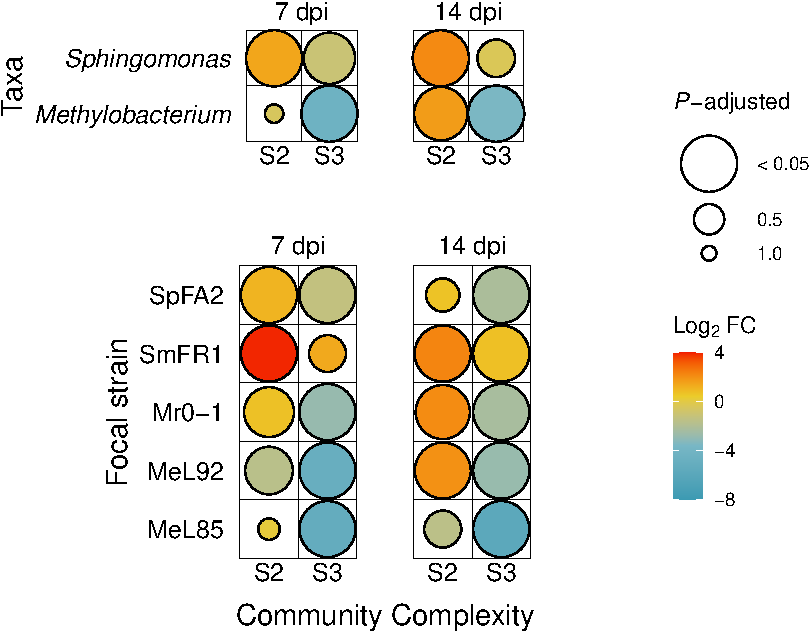
\includegraphics{results1_bacdensity_communitycomplexity_files/figure-latex/plot fig3b-1.pdf}

\begin{Shaded}
\begin{Highlighting}[]
\NormalTok{plt.sup1}
\end{Highlighting}
\end{Shaded}

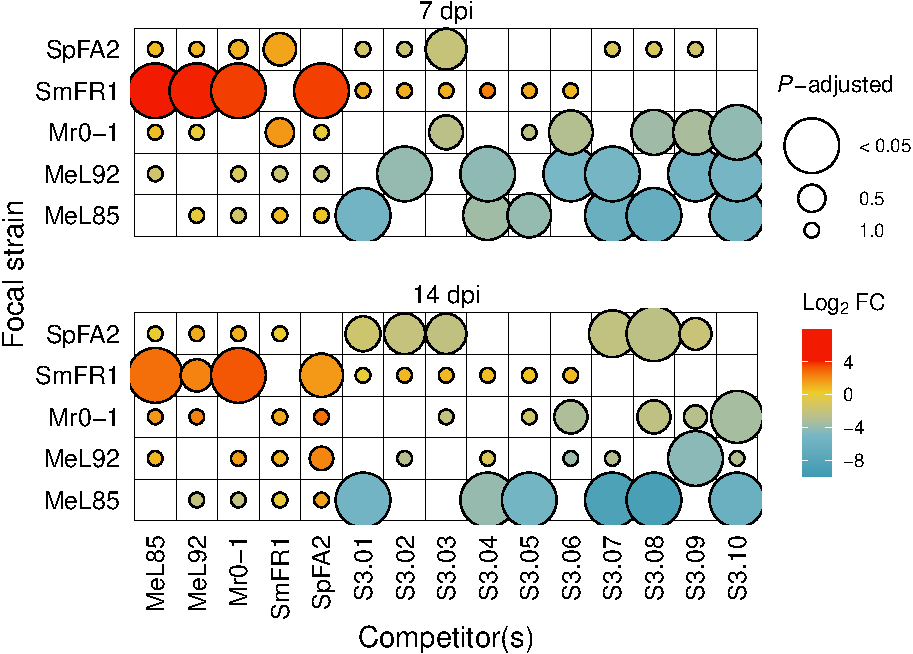
\includegraphics{results1_bacdensity_communitycomplexity_files/figure-latex/plot sup1-1.pdf}

The increase in population density in S2 was observed for populations of
both \emph{Methylobacterium} and \emph{Sphingomonas} (Fig. 3c). However,
within \emph{Methylobacterium}, MeL92 and Mr0-1 benefited the most in S2
(Fig. S1a). In particular, Mr0-1 consistently benefited from the
presence of individual \emph{Sphingomonas} strains. However, this effect
on methylobacteria was lost when a third competitor was present (S3),
regardless of the competitor's identity (Fig. S1b).

The increase in Sphingomonas population density in S2 was mainly
associated with an increase in SmFR1 populations (Fig. S1a), which was
higher in every S2 compared to C (Fig. S1b). For SpFA2, only a transient
effect was observed when this strain was paired with SmFR1 or MeL92;
however, both populations in each pair increased in density compared to
C, suggesting facilitative interactions. The decrease in population
density in S3 communities was observed only for Methylobacterium (Fig.
3c). The decrease in Methylobacterium population density was accompanied
by an increase in their coefficient of variation (Fig. 3d). The
increased coefficient of variation can be attributed to differences in
densities between the different Methylobacterium strains: MeL85 was most
impacted and had the lowest mean densities, while Mr0-1 and MeL92 were
less impacted (Fig. S1a). Within methylobacteria, the largest mean
difference was between MeL85 (1.58×105 CFU gFW-1) and Mr0-1 (2.51×106
CFU gFW-1) in S3 (t546 = 11.94, p \textless{} 0.001). However, the
largest mean differences were observed between MeL85 and SmFR1 (75.75×,
t894 = 25.79, p \textless{} 0.001) and with SpFA2 (73.13×, t894 = 25.58,
p \textless{} 0.001) in S3. In general, the decrease in each
Methylobacterium population density was observed for every S3 community
(Fig. S1b). These results indicate that bacterial taxa differentially
respond to community complexity in the phyllosphere and that
methylobacteria are more affected compared to sphingomonads.

\end{document}
